\documentclass{standalone}
\usepackage{tikz}
\usetikzlibrary{patterns, positioning}


\begin{document}
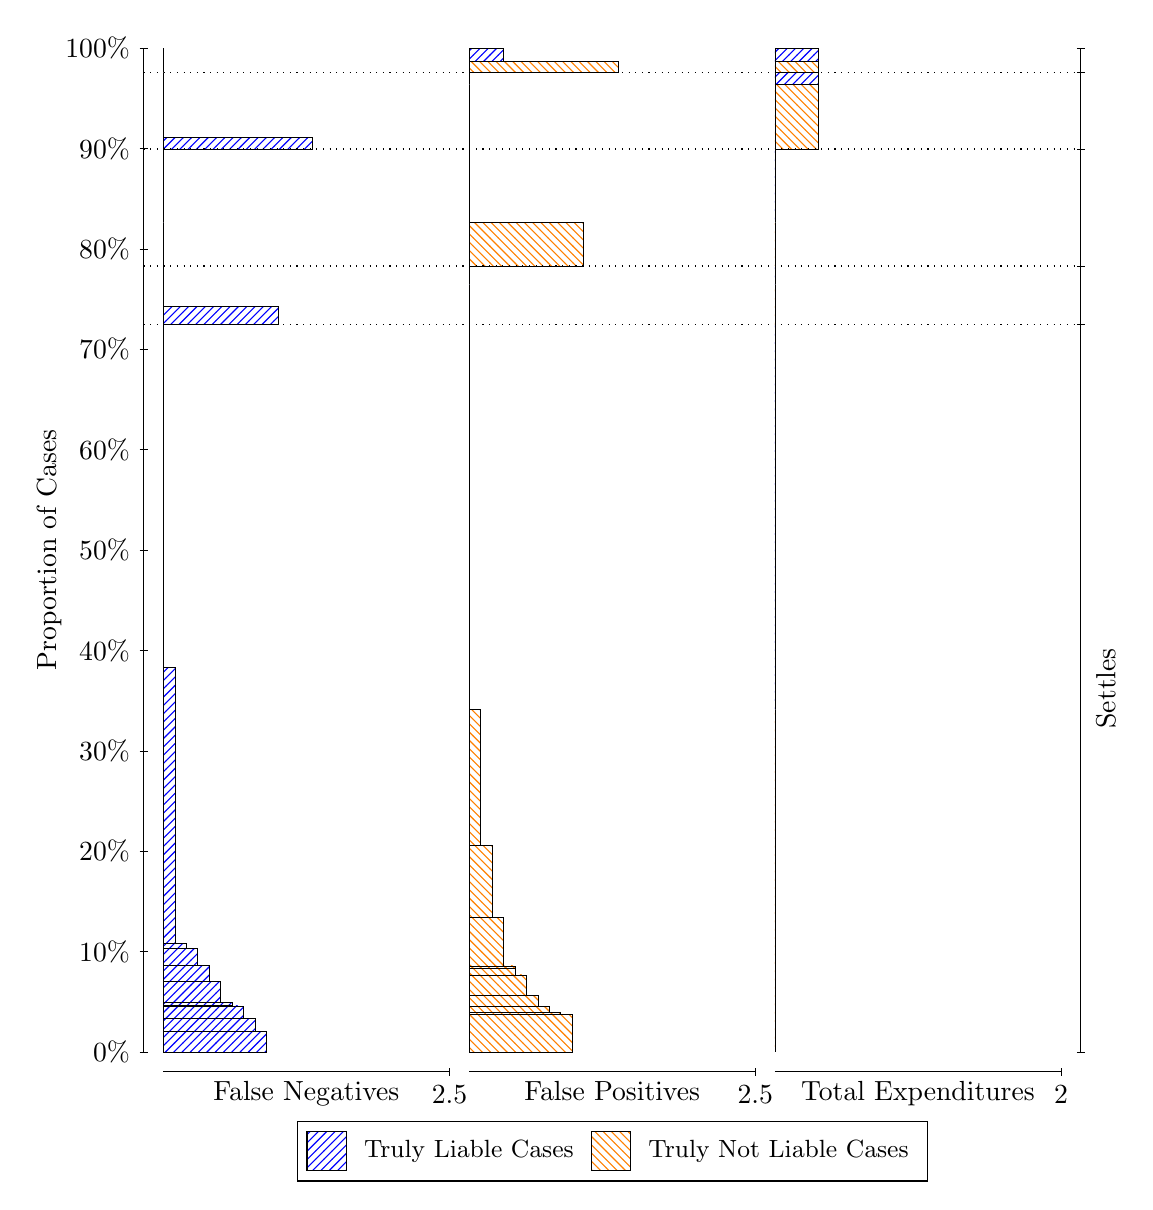
\begin{tikzpicture}
\draw[black, very thin] (1.5,1.75) -- (1.5,14.5);
\node[rotate=90, text=black, anchor=center] at (0.3, 8.125) {Proportion of Cases};
\draw[black, very thin] (1.45,1.75) -- (1.55,1.75);
\node[text=black, anchor=east] at (1.45, 1.75) {0\%};
\draw[black, very thin] (1.45,3.025) -- (1.55,3.025);
\node[text=black, anchor=east] at (1.45, 3.025) {10\%};
\draw[black, very thin] (1.45,4.3) -- (1.55,4.3);
\node[text=black, anchor=east] at (1.45, 4.3) {20\%};
\draw[black, very thin] (1.45,5.575) -- (1.55,5.575);
\node[text=black, anchor=east] at (1.45, 5.575) {30\%};
\draw[black, very thin] (1.45,6.85) -- (1.55,6.85);
\node[text=black, anchor=east] at (1.45, 6.85) {40\%};
\draw[black, very thin] (1.45,8.125) -- (1.55,8.125);
\node[text=black, anchor=east] at (1.45, 8.125) {50\%};
\draw[black, very thin] (1.45,9.4) -- (1.55,9.4);
\node[text=black, anchor=east] at (1.45, 9.4) {60\%};
\draw[black, very thin] (1.45,10.675) -- (1.55,10.675);
\node[text=black, anchor=east] at (1.45, 10.675) {70\%};
\draw[black, very thin] (1.45,11.95) -- (1.55,11.95);
\node[text=black, anchor=east] at (1.45, 11.95) {80\%};
\draw[black, very thin] (1.45,13.225) -- (1.55,13.225);
\node[text=black, anchor=east] at (1.45, 13.225) {90\%};
\draw[black, very thin] (1.45,14.5) -- (1.55,14.5);
\node[text=black, anchor=east] at (1.45, 14.5) {100\%};

\draw[black, very thin] (13.4,1.75) -- (13.4,14.5);
\draw[black, very thin] (13.35,1.75) -- (13.45,1.75);
\node[anchor=west] at (13.35, 1.75) {};
\draw[black, very thin] (13.35,10.986) -- (13.45,10.986);
\node[anchor=west] at (13.35, 10.986) {};
\draw[black, very thin] (13.35,11.732) -- (13.45,11.732);
\node[anchor=west] at (13.35, 11.732) {};
\draw[black, very thin] (13.35,13.218) -- (13.45,13.218);
\node[anchor=west] at (13.35, 13.218) {};
\draw[black, very thin] (13.35,14.187) -- (13.45,14.187);
\node[anchor=west] at (13.35, 14.187) {};
\draw[black, very thin] (13.35,14.5) -- (13.45,14.5);
\node[anchor=west] at (13.35, 14.5) {};

\draw[black, very thin, pattern color=blue, pattern=north east lines] (1.75,1.75) rectangle (3.058,2.0146);
\draw[black, very thin, pattern color=blue, pattern=north east lines] (1.75,2.0146) rectangle (2.9127,2.1774);
\draw[black, very thin, pattern color=blue, pattern=north east lines] (1.75,2.1774) rectangle (2.7673,2.3353);
\draw[black, very thin, pattern color=blue, pattern=north east lines] (1.75,2.3353) rectangle (2.622,2.34);
\draw[black, very thin, pattern color=blue, pattern=north east lines] (1.75,2.34) rectangle (2.622,2.3799);
\draw[black, very thin, pattern color=blue, pattern=north east lines] (1.75,2.3799) rectangle (2.4767,2.6472);
\draw[black, very thin, pattern color=blue, pattern=north east lines] (1.75,2.6472) rectangle (2.3313,2.8498);
\draw[black, very thin, pattern color=blue, pattern=north east lines] (1.75,2.8498) rectangle (2.186,3.0636);
\draw[black, very thin, pattern color=blue, pattern=north east lines] (1.75,3.0636) rectangle (2.0407,3.133);
\draw[black, very thin, pattern color=blue, pattern=north east lines] (1.75,3.133) rectangle (1.8953,6.6366);
\draw[black, very thin, pattern color=orange, pattern=north west lines] (1.75,6.6366) rectangle (1.75,10.986);
\draw[black, very thin, pattern color=blue, pattern=north east lines] (1.75,10.986) rectangle (3.2033,11.223);
\draw[black, very thin, pattern color=orange, pattern=north west lines] (1.75,11.223) rectangle (1.75,11.732);
\draw[black, very thin, pattern color=orange, pattern=north west lines] (1.75,11.732) rectangle (1.75,12.283);
\draw[black, very thin, pattern color=blue, pattern=north east lines] (1.75,12.283) rectangle (1.75,13.218);
\draw[black, very thin, pattern color=blue, pattern=north east lines] (1.75,13.218) rectangle (3.6393,13.37);
\draw[black, very thin, pattern color=orange, pattern=north west lines] (1.75,13.37) rectangle (1.75,14.187);
\draw[black, very thin, pattern color=orange, pattern=north west lines] (1.75,14.187) rectangle (1.75,14.335);
\draw[black, very thin, pattern color=blue, pattern=north east lines] (1.75,14.335) rectangle (1.75,14.5);
\draw[black, very thin, pattern color=orange, pattern=north west lines] (5.6333,1.75) rectangle (6.9413,2.2284);
\draw[black, very thin, pattern color=orange, pattern=north west lines] (5.6333,2.2284) rectangle (6.796,2.2536);
\draw[black, very thin, pattern color=orange, pattern=north west lines] (5.6333,2.2536) rectangle (6.6507,2.3322);
\draw[black, very thin, pattern color=orange, pattern=north west lines] (5.6333,2.3322) rectangle (6.5053,2.4654);
\draw[black, very thin, pattern color=orange, pattern=north west lines] (5.6333,2.4654) rectangle (6.36,2.7287);
\draw[black, very thin, pattern color=orange, pattern=north west lines] (5.6333,2.7287) rectangle (6.2147,2.8167);
\draw[black, very thin, pattern color=orange, pattern=north west lines] (5.6333,2.8167) rectangle (6.2147,2.8447);
\draw[black, very thin, pattern color=orange, pattern=north west lines] (5.6333,2.8447) rectangle (6.0693,3.4571);
\draw[black, very thin, pattern color=orange, pattern=north west lines] (5.6333,3.4571) rectangle (5.924,4.3747);
\draw[black, very thin, pattern color=orange, pattern=north west lines] (5.6333,4.3747) rectangle (5.7787,6.0993);
\draw[black, very thin, pattern color=blue, pattern=north east lines] (5.6333,6.0993) rectangle (5.6333,10.986);
\draw[black, very thin, pattern color=orange, pattern=north west lines] (5.6333,10.986) rectangle (5.6333,11.495);
\draw[black, very thin, pattern color=blue, pattern=north east lines] (5.6333,11.495) rectangle (5.6333,11.732);
\draw[black, very thin, pattern color=orange, pattern=north west lines] (5.6333,11.732) rectangle (7.0867,12.283);
\draw[black, very thin, pattern color=blue, pattern=north east lines] (5.6333,12.283) rectangle (5.6333,13.218);
\draw[black, very thin, pattern color=orange, pattern=north west lines] (5.6333,13.218) rectangle (5.6333,14.034);
\draw[black, very thin, pattern color=blue, pattern=north east lines] (5.6333,14.034) rectangle (5.6333,14.187);
\draw[black, very thin, pattern color=orange, pattern=north west lines] (5.6333,14.187) rectangle (7.5227,14.335);
\draw[black, very thin, pattern color=blue, pattern=north east lines] (5.6333,14.335) rectangle (6.0693,14.5);
\draw[black, very thin, pattern color=orange, pattern=north west lines] (9.5167,1.75) rectangle (9.5167,6.0993);
\draw[black, very thin, pattern color=blue, pattern=north east lines] (9.5167,6.0993) rectangle (9.5167,10.986);
\draw[black, very thin, pattern color=orange, pattern=north west lines] (9.5167,10.986) rectangle (9.5167,11.495);
\draw[black, very thin, pattern color=blue, pattern=north east lines] (9.5167,11.495) rectangle (9.5167,11.732);
\draw[black, very thin, pattern color=orange, pattern=north west lines] (9.5167,11.732) rectangle (9.5167,12.283);
\draw[black, very thin, pattern color=blue, pattern=north east lines] (9.5167,12.283) rectangle (9.5167,13.218);
\draw[black, very thin, pattern color=orange, pattern=north west lines] (9.5167,13.218) rectangle (10.062,14.034);
\draw[black, very thin, pattern color=blue, pattern=north east lines] (9.5167,14.034) rectangle (10.062,14.187);
\draw[black, very thin, pattern color=orange, pattern=north west lines] (9.5167,14.187) rectangle (10.062,14.335);
\draw[black, very thin, pattern color=blue, pattern=north east lines] (9.5167,14.335) rectangle (10.062,14.5);
\draw[black, dotted] (1.5,10.986) -- (13.4,10.986);
\draw[black, dotted] (1.5,11.732) -- (13.4,11.732);
\draw[black, dotted] (1.5,13.218) -- (13.4,13.218);
\draw[black, dotted] (1.5,14.187) -- (13.4,14.187);
\draw[black, very thin] (1.75,1.5) -- (5.3833,1.5);
\node[text=black, anchor=north] at (3.5667, 1.5) {False Negatives};
\draw[black, very thin] (5.3833,1.45) -- (5.3833,1.55);
\node[text=black, anchor=north] at (5.3833, 1.45) {2.5};

\draw[black, very thin] (5.6333,1.5) -- (9.2667,1.5);
\node[text=black, anchor=north] at (7.45, 1.5) {False Positives};
\draw[black, very thin] (9.2667,1.45) -- (9.2667,1.55);
\node[text=black, anchor=north] at (9.2667, 1.45) {2.5};

\draw[black, very thin] (9.5167,1.5) -- (13.15,1.5);
\node[text=black, anchor=north] at (11.333, 1.5) {Total Expenditures};
\draw[black, very thin] (13.15,1.45) -- (13.15,1.55);
\node[text=black, anchor=north] at (13.15, 1.45) {2};

\node[text=black, centered, rotate=90] at (13.72, 6.368) {Settles};





\draw (7.449999999999999,1.5) node[draw=none] (baseCoordinate) {};
\begin{scope}[align=center]
        \matrix[scale=0.5, draw=black, below=0.5cm of baseCoordinate, nodes={draw}, column sep=0.1cm]{
            \node[rectangle, draw, minimum width=0.5cm, minimum height=0.5cm, pattern color=blue, pattern=north east lines] {}; &
            \node[draw=none, font=\small, text=black] (B) {Truly Liable Cases}; &
            \node[rectangle, draw, minimum width=0.5cm, minimum height=0.5cm, pattern color=orange, pattern=north west lines] {}; &
            \node[draw=none, font=\small, text=black] (B) {Truly Not Liable Cases}; \\
            };
\end{scope}

\end{tikzpicture}
\end{document}